\documentclass[20pt,margin=1in,innermargin=-4.5in,blockverticalspace=-0.25in]{tikzposter}
\geometry{paperwidth=33.11in,paperheight=46.81in} %A0
% \geometry{paperheight=33.11in,paperwidth=23.4in} %A1
\usepackage[utf8]{inputenc}
\usepackage{amsmath}
\usepackage{amsfonts}
\usepackage{amsthm}
\usepackage{amssymb}
\usepackage{mathrsfs}
\usepackage{graphicx}
\usepackage{amsrefs}
\newcommand{\mycomment}[1]{}
\graphicspath{ {images/} }
\usepackage[export]{adjustbox}
\usepackage{enumitem}
%\usepackage[backend=biber, style=numeric]{biblatex}
\usepackage{ubtheme}
\makeatletter
\setlength{\TP@visibletextwidth}{31.0in}
\setlength{ \TP@visibletextheight}{45in}
\makeatother
\usepackage{mwe} % for placeholder images
\usepackage{bm}
\usepackage{bbm}
\definecolor{bristolred}{HTML}{B01C2E}
%\addbibresource{refs.bib}

% set theme parameters
\tikzposterlatexaffectionproofoff
\usetheme{UBTheme}
\usecolorstyle{UBStyle}
\usepackage{comment}
%\usepackage{ragged2e}
\usepackage{mathtools}
%\usepackage[numbers]{natbib}
\usepackage{amsmath,amssymb,amsthm,mathrsfs}
%\usepackage{xfrac}
\usepackage{xcolor}
\usepackage{amsfonts}
\usepackage{tikz}
\usepackage{pgfplots}
\pgfplotsset{compat=newest}
\usetikzlibrary{decorations.markings}
%\usepackage{graphicx}
%\usepackage[english]{babel}
%\usepackage[utf8x]{inputenc}
\usepackage[scaled]{helvet}
\renewcommand\familydefault{\sfdefault} 
\renewcommand{\vec}[1]{\bm{#1}}
\newcommand{\Tr}{\text{Tr}}
\usepackage[T1]{fontenc}
\newcommand{\qrfac}[2]{{\left({#1}\right)_{#2}}} % suppressing q
\newcommand{\pqrfac}[3]{{\left({#1};#3\right)_{#2}}}
\newcommand{\prodl}{\prod\limits}


\title{\parbox{0.95\linewidth}{Generalised Stokes Theorem}}
\author{\textbf{Vishnu Varadarajan}}
\institute{Ashoka University Math Apprenticeship Program, Ashoka University}

\titlegraphic{
\includegraphics[width=0.2\textwidth]{Ashoka_University_logo_with_wordmark.png}}

\tikzset{arrmark/.style={postaction={decorate,decoration={markings,
mark=at position #1/11-0.1/11 with {\arrow[orange]{<};},
mark=at position #1/11+0.1/11 with {\arrow[orange]{>};}}}}}

\begin{document}
\maketitle
\centering
    \begin{columns}
        \column{0.5}
        \block{Context}{
            \begin{itemize}
                \item Gauss was studying surfaces, and wanted to define curvature in a way that was independent of the $3-$dimensional space that the surface is embedded in. The vector calculus view of surfaces is an extrinsic view. But there is also an intrinsic geometry of these surfaces.
                \begin{center}
                    \begin{tikzpicture}
                        \draw[<->, thin] (-10,0) to (-5,0) node[above left=10pt] {$\mathbb{R}$};
                        \draw[red, thick] (-9,0) node{$\circ$} to (-6,0) node{$\circ$};

                        \draw[<->, thin] (-4,0) to (1,0) node[above left=10pt] {$\mathbb{R}^2$};
                        \draw[<->, thin] (-1.5,-2.5) to (-1.5, 2.5);
                        \node[red] (A) at (-3,1.5) {$\circ$};
                        \node[red] (B) at (0,-1.5) {$\circ$};
                        \draw[red, bend right] (-3,1.5) to (-1.5,0);
                        \draw[red, bend right] (0,-1.5) to (-1.5,0);
                    \end{tikzpicture} \quad
                    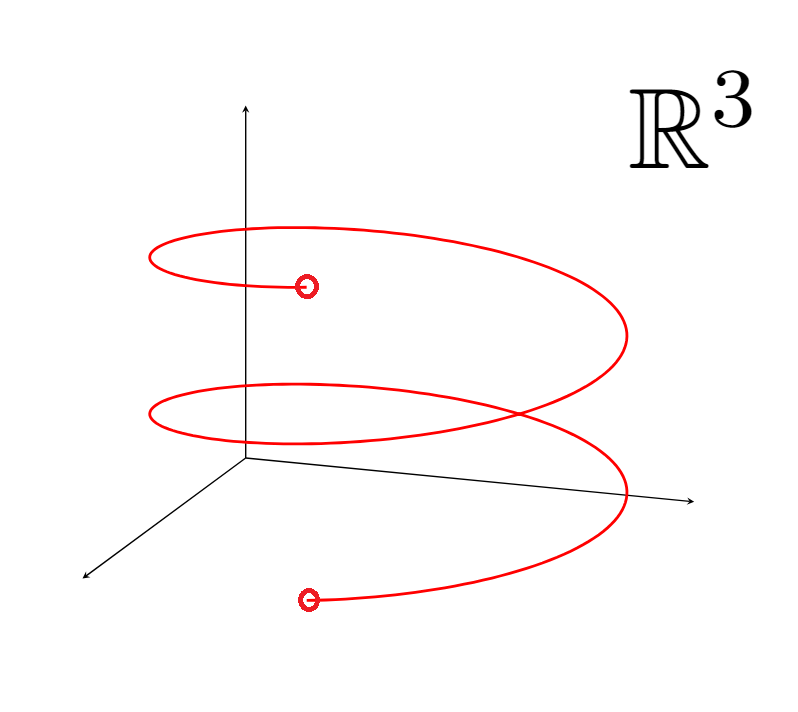
\includegraphics[scale=0.4]{lineinr3.png} 
                \end{center}
                This intrinsic view of surfaces, is developed in the theory of manifolds.
                
                \item The generalised stokes theorem is an analog to the fundamental theorem of calculus, in the setting of manifolds. The fundamental theorem of calculus states:
                \begin{center}
                    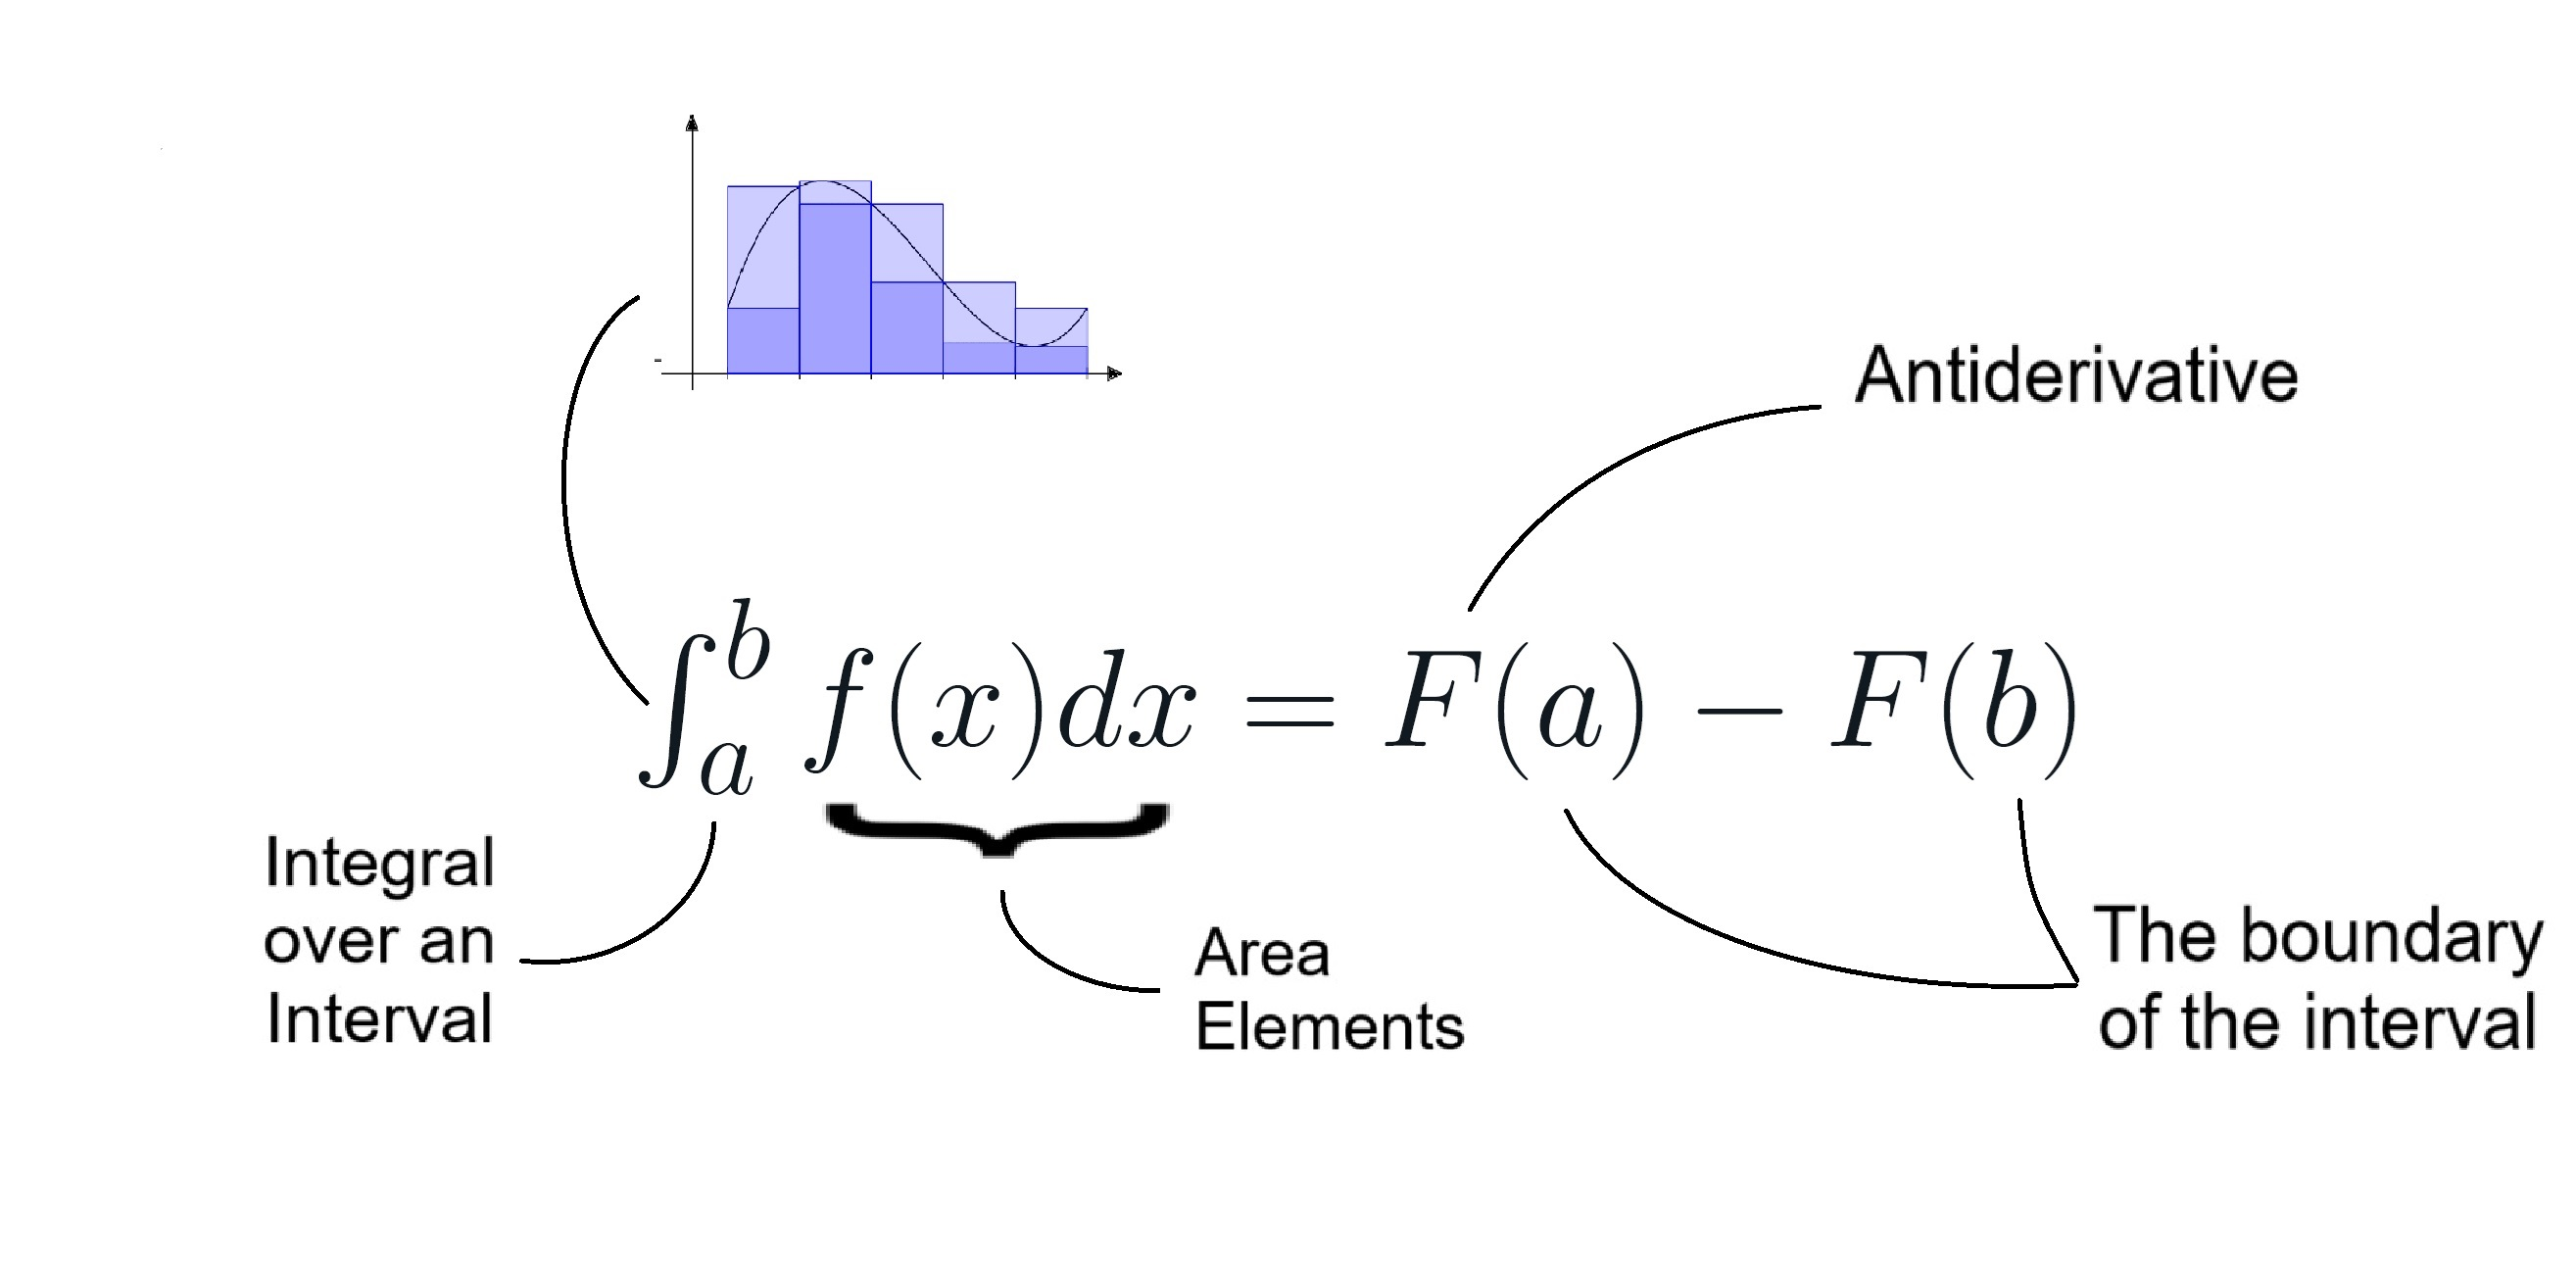
\includegraphics[scale=0.45]{ftc.jpg}
                \end{center}
            \end{itemize}
        }
        \block{Manifolds}{
            \begin{itemize}
                \item Manifolds are a topological space such that each point is locally homeomorphic to an open set in a Euclidean space. For example, circles, spheres, torus, m\"obius strip etc.
                \begin{center}
                    % 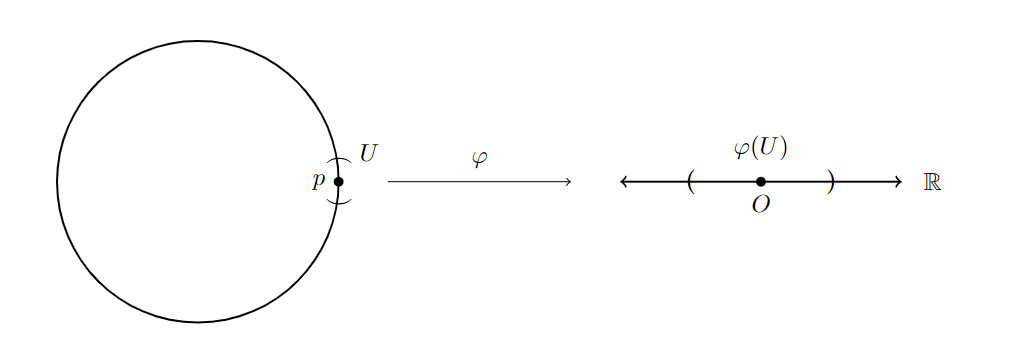
\includegraphics[scale=0.9]{circ1man.png}
                    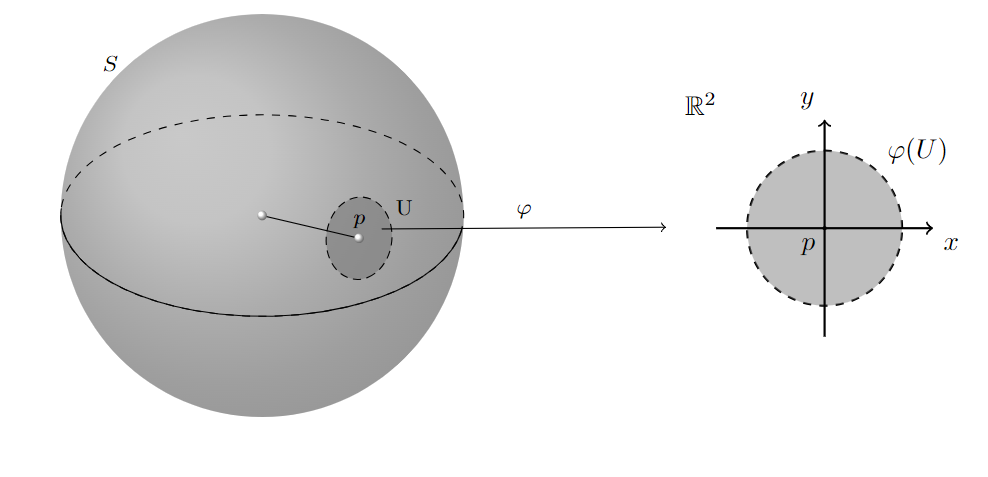
\includegraphics[scale=1]{sphere2man.png}
                \end{center}
                In the above, the neighborhood paired with the homeomorphism $(U,\varphi)$ is called a \textit{chart}. Because at all points this manifold resembles a Euclidean space, a collection of these charts for neighborhoods of each point on the manifold, is given the term \textit{Atlas}.
                \item smooth manifolds.
                \item There are surfaces that dont fully fit into this definition like the hemisphere. The neighborhood of a point on its boundary is not homeomorphic to a Euclidean space, because it is not an open set. For this rather than the entire euclidean space, we restrict the domain of the homeomorphism to the Euclidean Half space. Such structures are called \textit{Manifolds with boundary}
                \begin{center}
                    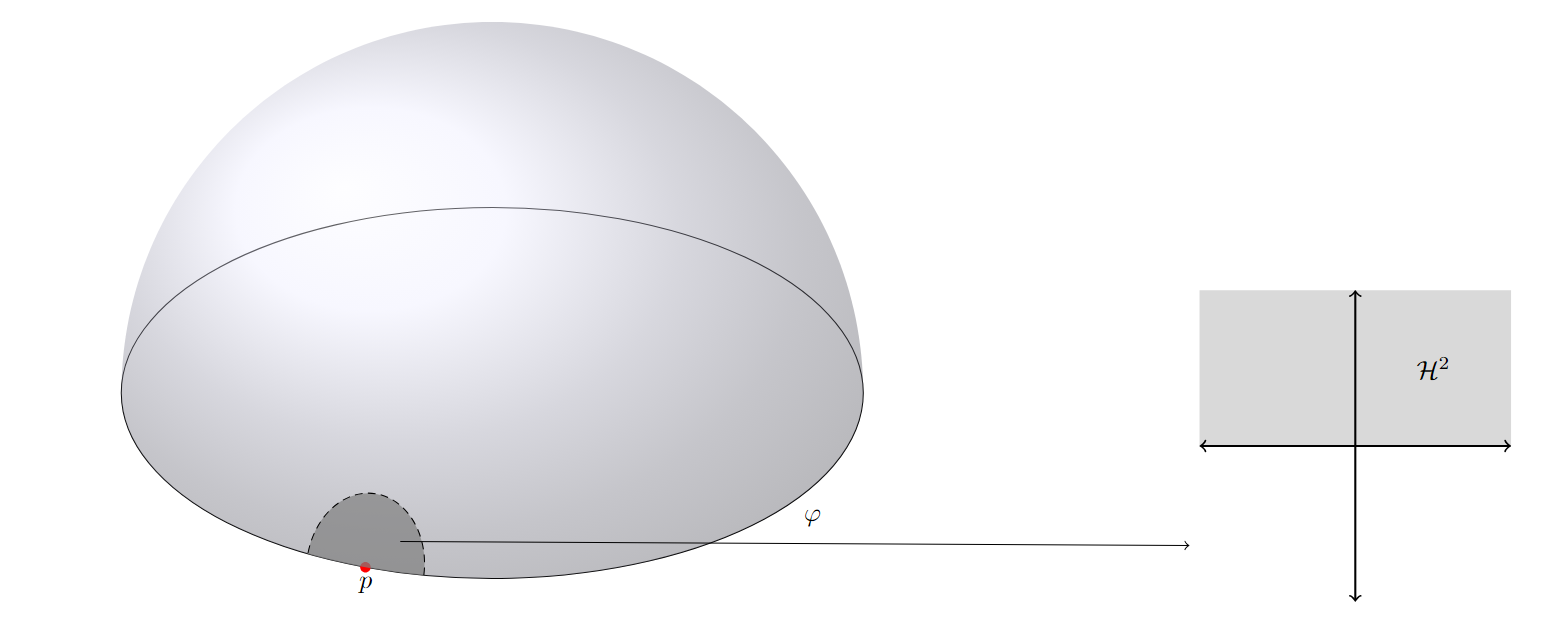
\includegraphics[scale=0.45]{manwbound.png}
                \end{center}
                \item Tangent Space: Recall the view of tangents as the direction of motion on a path on the surface. This is the idea behind the tangent space. We consider paths on the manifold and the directional derivative operator along these paths on functions on the manifold as the tangent vectors. 
                \begin{center}
                    
                        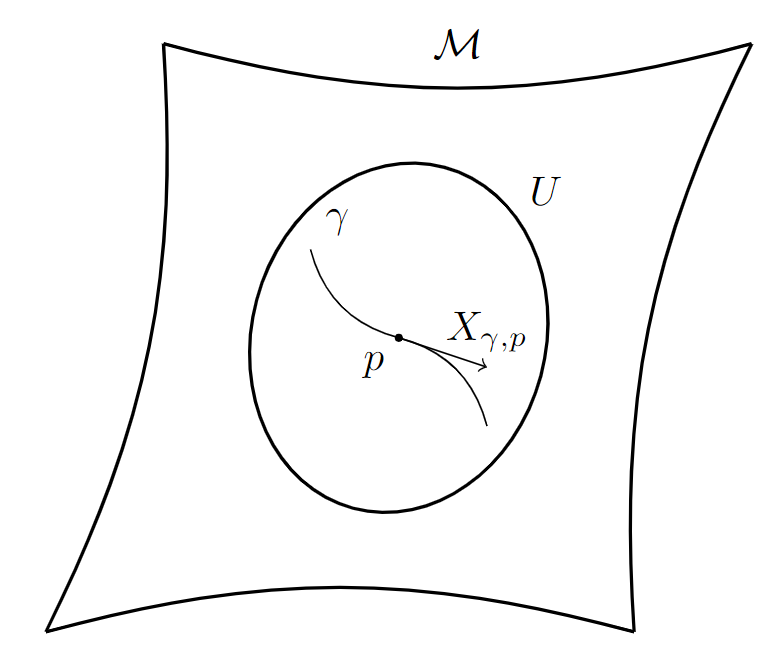
\includegraphics[scale=0.4]{tangentvec.png} 
                        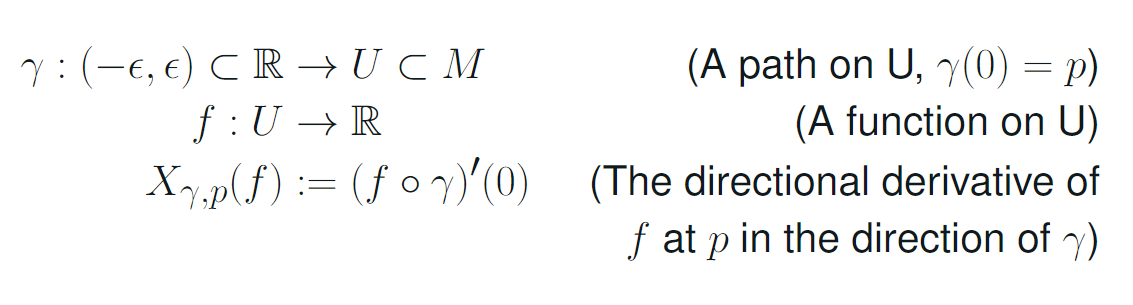
\includegraphics[scale=0.75]{tanvecdetails.png}
                \end{center}
            \end{itemize}
        }

        \column{0.5}
        \block{Differential Forms}{
        \begin{itemize}
            \item Tensors: $k-$linear, real valued functions, $V^k \to \mathbb{R}$. Examples: the dot product, a two tensor, the determinant, a $k-$tensor.
            \\
            Tensor product: combines a $k$ and an $l$ tensor to give a $k+l$ tensor. Defined as 
            \[
                (K \otimes L)(v_1, v_2, \dots, v_{k+l}) = K(v_1 \dots v_k)\cdot L(v_k+1, \dots, v_{k+l})
            \]


            \item The dual of a vector space $V$ is the space of linear, real valued functions on $V$. This is denoted $V^*$. So it is also the space of 1-tensors on $V$. The dual space is isomorphic to the original vector space.
            \item Forms on $\mathbb{R}^n$: A $k-$form on $\mathbb{R}^n$ is an alternating $k-$tensor 
            \item forms on manifold, 1 forms as cotangent vetors
            \item exterior derivative
            \item pull backs
        \end{itemize}
        }
        \block{Integration}{
            \begin{itemize}
                \item integral of forms on Rn
                \item partitions of unity
                \item integral of forms on M
                \item change of variables
                \item integral of forms on Rn
                \item partitions of unity
                \item integral of forms on M
                \item change of variables
            \end{itemize}
        }
        \block{Generalised Stokes Theorem}{
            statement, visual importance
        }
    \end{columns}
\end{document}